\documentclass[lmodern, utf8, seminar]{fer}
\usepackage{booktabs}
\usepackage{graphicx}
\usepackage{float}

\graphicspath{ {images/} }

\begin{document}
\nocite{*}



\title{Suparnički generativni modeli za prevođenje slika}

\author{Krešimir Vukić}
\voditelj{prof.~dr.~sc.~Siniša Šegvić}

\maketitle


\tableofcontents



\chapter{Uvod}
Razvojem tehnika namjenjenih identifikaciji i analizi slika, logični sljedeći korak unutar područja računalnog vida bio je osmišljavanje algoritama kojima bi se omogućila reprodukcija vizualnih sadržaja. 
\newline

Generiranje slika na temelju skice, prijenos stilova i rekonstrukcija fotografije neke su od primjena dotičnog problema. Najznačajniji pomak u tome području ostvarili su Goodfellow et al. 2014. g. \cite{goodfellow2014generative} osmišljavanjem generativhin suparničkih modela čiji tipičan cilj je učenje funkcije preslikavanja iz prostora latentnih varijabli na željenu distribuciju.

Dobivena distribucija, osim za generiranje novih primjera, primjenjiva je i na rješavanje prvotno navedenih problema identifikacije značajki na postojećim slikama. Ta fleksibilnost čini ovaj algoritam izuzetno popularnim za istraživanje što je rezultiralo njegovim mnogobrojnim modifikacijama i poboljšanjima.
\newline

Ovim radom istražiti će se različita proširenja kojima se ti modeli prilagođavaju specifičnim problemima, njihove karakteristike i primjene.

\chapter{Duboke mreže}
Duboke neuronske mreže zadnjih godina izuzetno su popularne u rješavanju klasifikacijskih problema i pronalaženju uzoraka. Tome je zaslužna prednost koju imaju naspram klasičnih pristupa, a koja se očituje u vidu mogućnosti da samostalno pronalaze bitne značajke u podatcima te na temelju njih i tražena rješenja.

Slojevit pristupu rastavljanja podataka na jednostavnije građevne jedinice čini ih posebice prigodnima za radu sa problemima hijerarhijske prirode poput slika. 
\newline

\section{Konvolucija}
Konvolucijske mreže osmišljene su s ciljem dohvata lokalnih relacija među podatcima koje se posebice očituju pri radu sa slikama. Naime, ukoliko želimo analizirati malenu značajku na slici, nepoželjno je da njena pozadina ili lokacija unutar slike utječe na nju samu. 

Ideja konvolucije je da se kao ulaz u neurone sljedećeg sloja dovede više vrijednosti s prethodnog što je prikazano slikom \ref{fig:convolution}. To se odvija tako da se unaprijed definiran kvadrat pomiče (konvoluira) po ulaznim podatcima i tako određuje mapiranje na sljedeći sloj. Rezultat tog procesa je da pridodajemo veću važnost pikselima u neposrednoj okolini istraživanog područja.
\newline

\begin{figure}[H]
    \centering
    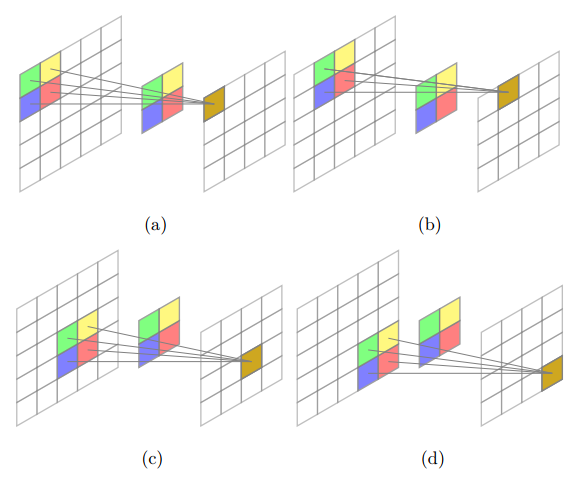
\includegraphics[width=0.8\textwidth]{convolution}
    \caption{Proces konvolucije}
    \label{fig:convolution}
\end{figure}

\section{Primjer konvolucijske mreže}
Nizanjem konvolucijskih slojeva dobivamo arhitekturu u kojoj je svaki sloj zadužen za jednostavniji potproblem sljedećeg sloja. Na slici \ref{fig:dnn} prikazana je duboka neuronska mreža s 5 konvolucijskih slojeva među kojima se odvija sažimanje maksimalnom vrijednošću te dva sloja potpune povezanosti.
\newline

\begin{figure}[H]
    \centering
    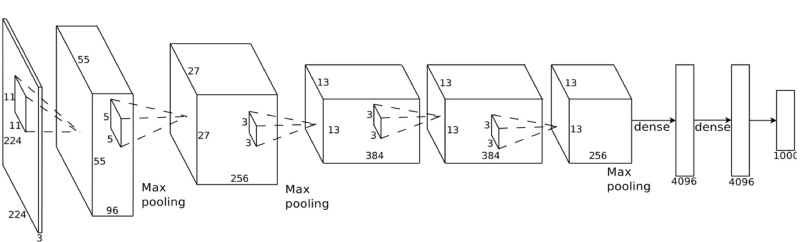
\includegraphics[width=0.9\textwidth]{dnn}
    \caption{Primjer duboke neuronske mreže}
    \label{fig:dnn}
\end{figure}

\chapter{Generativni suparnički modeli (GAN-ovi)}
\section{Generativni naspram diskriminativnih algoritama}
Dvije temeljne skupine koijima dijelimo algoritme za učenje su diskriminativni i generativni.
Nazivi tih algoritama dolaze izravno iz vrste problema koji riješavaju: 
\newline

% setting item mark to bullet
\renewcommand{\labelitemi}{\textbullet}
\begin{itemize} 
\item Diskriminativni modeli baziraju se na modeliranju isključivo pomoću ulaznih varijabli koje direktno mapiraju na ciljne vrijednosti i time uče uvjetnu vjerojatnost $p(Y|X)$. Ne stvaraju puno pretpostavki o podložnoj distribuciji, no vrlo su ovisni o kvalitetnim podatcima. 
%Dobiveni model svrstava podatke u ciljne klase s određenom vjerojatnošću.

\item Generativni modeli riješavaju problem kako dobiti $X$ uz dani $Y$, tj. pokušavaju naučiti distribuciju pojedinih klasa $p(X\mid Y)$.
\newline
\end{itemize}

Drugim riječima, dok diskriminativni modeli pokušavaju pronaći granicu između klasa, generativni modeliraju distribucije pojedinih klasa na temelju kojih mogu uzorkovati nove primjere.
\newline

\section{Suparnički modeli}
U praksi se pokazalo kako diskriminativni modeli postižu bolje rezultate od generativnih. Iako je očito da su generativni algoritmi svestranije naravi od diskriminativnih, to dolazi sa neizbježnim povećanjem složenosti koja proizlazi iz toga što se pronalazak ciljne distribucije u dubokim hijerarhijskim podatcima sastoji od aproksimiranja problema čija riješenja matematički nije moguće izvesti \cite{goodfellow2014generative}. Bez toga, nije moguće ni podesiti model da radi pri svom optimumu. Odgovor na predstavljenu složenost pronađen je u suparničkim modelima čiji rad se bazira na istovremenom učenju dvije podmreže. Ovisno o implementaciji, mreža takve arhitekture u stanju je kopirati distribuciju širokog spektra podataka: slika, govora, muzike, pa čak i pisanih zapisa.
\newline

\section{Rad GAN-a}
Ideja generativnih suparničkih modela je da se istovremeno uče dvije mreže.
Pola mreže (generator $G$) bavi se stvaranjem novih podataka iz neke jednostavne distribucije $Z$ s ciljem da stvoreni podatci budu čim sličniji stvarnima. Paralelno s njegovim radom, druga polovica (diskriminator $D$) pokušava evaluirati koliko su uzorci $G(Z)$ slični stvarnim podatcima $Y$. Drugim riječima, dok $G$ pokušava minimizirati izlaz $D-a$, $D$ ga pokušava maksimizirati.
Cijeli proces usporedljiv je s poslovima detektiav i kriminalca. Jedna strana u bavi se falsifikacijom dokaza, a druga analizom njihove autentičnosti.
\newline

Koraci rada GANa:
\begin{enumerate} 
\item generator $G$ iz nasumičnih brojeva (šum) $Z$ stvara sliku $G(Z)$
\item ta slika se dovodi na ulaz diskriminatora $D$ uz skup stvarnih slika iz podatkovnog skupa $Y$
\item diskriminator $D$ određuje postotak vjerojatnosti da je slika $G(Z)$ prava
\end{enumerate}

\section{GAN-ovi naspram autoenkodera}


\chapter{Uvjetne generativne mreže}
\section{Generalizacija problema prevođenja slike}
Isola et al. \cite{isola2017image} predložili su uvjetne generativne mreže kao generalno rješenje problema prevođenja slike. Svojstvene su po učenju ne samo funkcije prijenosa između slika već i funkcije gubitka nad kojom se ona trenira.
Dok se u drugim modelima ona ručno zadaje, pristup u kojem se ona uči omogučuje generalizaciju nad setovima problema koji bi u suprotnom zahtijevali vrlo drugačije formulacije gubitka.
\newline

\section{Pristup prevođenju slike}
Analogno prevođenju teksta u drugi jezik zadržavajući određeni kontekst, prevođenje slike odnosi se na translaciju scene u drugačiju reprezentaciju. To se odnosi na mnogobrojne probleme za koje postoje zasebne metode riješavanja poput izmjene pozadine, lica ili promjene boje. No, u srži svih njih može se prepoznati jedinstven problem: naći funkciju preslikavanja piksela u piksel. Tokom učenja, lošim definiranjem te funkcije, nikad nećemo dobiti realistične rezultate. GANovi pristupaju tome tako da odbacuju sva riješenja koja se mogu razlikovati od stvarnosti generirajući slike $y$ iz nasumičnog šuma $z$ : $G: z \rightarrow y$. Poboljšanje nad tom metodom dobivamo uz uvjetovanje ulaznih podataka, tj. uz dodavanja uvjeta na šum da mora sličiti stvarnoj distribuciji. To se postiže dodavanjem slike $x$ slične željenoj na ulaz sustava $G: {x,z} \rightarrow y$ \cite{isola2017image}.

\section{Primjena}
Neke od mogućnosti uvjetnih GAN-ova su sinteza fotorealističnih slika iz skica, generiranje objekata na temelju njihovih obruba te bojanje crno bijelih fotografija.



\chapter{Translacija bez uparenih primjera za učenje}
\section{Kružni GAN-ovi}

\subsection{Prednosti}
Većina postojećih algoritama korištenih u računalnom vidu ovisi o postojanju velikih podatkovnih setova označenih parova slika. No, za mnoge probleme takvi podatci nisu dostupni, a u takvim situacijama primjenu nalaze kružni GANovi.
\newline

\subsection{Rad CycleGAN-a}
Temelj njihovog rada je uz da uz učenje funkcije $G: X \rightarrow Y$, istovremeno uče njen inverz $F: X \rightarrow Y$ pomoću gubitka cikličke dosljednosti: $F(G(X)) \approx X$ i obrnuto.

\section{Multimodalna translacija (MUNIT)}
Druge metode nenadziranog učenja translacije ne uzimaju u obzir da je uvjetna distribucija preslikavanja slika između dvije domene inherentno multimodalna [huang2018multimodal] što kao poslijedicu ima da pri generiranju vrlo teško stvaraju vidljivo različite uzorke. MUNIT model pretpostavlja da se reprezentacija slike može rastaviti na značajke koje su domenski invarijantne te na one koje sadrže domenski specifična svojstva. Zatim se pri generiranju jednostavno domenski invarijantne značajke kombiniraju sa nasumičnim stilskim kodom uzorkovanim s ciljne domene.


\chapter{Prijenos stila}
\section{Očuvanje strukture}
Postojeće metode ograničene su izborom stilova koje mogu prenijeti te u realističnosti dobivenih rezultata. Pokušaji prijenosa stila koji mijenjaju vrijednost piksela unose sitne izmjene u linijama i teksturama što na rezultantnom sadržaju stvara dojam crteža, a gubi se realističnost fotografije. Uvjet koji se zbog toga postavlja na rad mreže je da mogže unositi izmjene isključivo na prostoru boja.

\section{Lokalizacija stila i očuvanje konteksta} \cite{luan2017deep}
Postoji još jedan faktor koji povećava kompleksnost cijelog procesa, a to je da se ciljano ponašanje prijenosa stila drži konteksta izmjene. Na primjer, ukoliko se na fotografiji nalaze livada i oblaci, modifikacije na livadi moraju biti povezane sa stilom livade na referentnoj slici, a ne da povuku stil sa oblaka. 



\chapter{Zaključak}
Generativni modeli tema su mnogobrojnih istraživanja i vrlo obečavajuća metoda učenja 'prirodnih' značajki podataka. Uz napretke koji se redovno postižu u njihovom unaprijeđenju, velika je vjerojatnost da će ubrzo biti u stanju generirati uzorke nerazlučive od stvarnosti. Time primjenu pronalaze u područjima poput stvaranja virtualnih svijetova bez ljudske intervencije, izvršavanja modifikacija nad slikama pomoću jednostavnog govora, regeneriranju oštećenih podataka ili stvaranju novih za buduća istraživanja.
\newline

...
Uvjetnim suparničkim mrežama pokazano je da osim što više nije potrebno ručno izvoditi funkcije preslikavanja, zadovoljavajuće rezultate možemo dobiti i ako dubokoj mreži prepustimo da sama nauči funkciju gubitka. To je velik korak prema široj adaptaciji ove tehnologije upravo zato što uklanja potrebu za inžinjerom i omogućava ljudima poput umjetnika i mladih znanstvenika da ju koriste samostalno.
...
\newline

\bibliographystyle{fer}
\bibliography{literatura}


\begin{sazetak}
Mnogi problemi u procesiranju slika odnose se na translaciju ulazne slike u željenu izlaznu. Većina današnjih arhitektura bazira se na generativnim suparničkim mrežama, nad kojima su osmišljena mnoga proširenja kako bi se prilagodila specifičnim problemima. Uvjetnim generativnim mrežama nije potrebno definirati funkciju gubitka jer ju mogu same naučiti, kružne generativne mreže sposobne su učenju translacije ne samo ulaznih u izlazne primjere nego i u drugom smjeru, a ograničavanjem mreže na translaciju unutar prostora boja obavljat će prijenos stila bez distorzije sadržaja slike. Ovim radom usporedit ću različite arhitekture, njihove karakteristike i primjene na problemima translacije slike u sliku.

\kljucnerijeci{image-to-image generation, style transfer, GANs, CycleGANs}
\end{sazetak}

\engtitle{Image to image generation using CycleGANs}
\begin{abstract}

\keywords{image-to-image generation, style transfer, GANs, CycleGANs}
\end{abstract}

\end{document}